\documentclass[tikz,border=8pt]{standalone}
\usepackage{tikz}
\usepackage{fontawesome5}
\usepackage{amsmath,amssymb}
\usetikzlibrary{arrows.meta,positioning,fit,backgrounds,calc,shadows,shapes.geometric}

\definecolor{civNavy}{RGB}{15, 34, 64}
\definecolor{civBlue}{RGB}{28, 80, 160}
\definecolor{civTeal}{RGB}{14, 130, 120}
\definecolor{civLightBlue}{RGB}{238, 245, 255}
\definecolor{civBorder}{RGB}{185, 210, 240}
\definecolor{civGold}{RGB}{217, 119, 6}
\definecolor{civGreen}{RGB}{22, 130, 80}
\definecolor{civDark}{RGB}{20, 28, 42}
\definecolor{cInput}{RGB}{240, 246, 255}
\definecolor{cStem}{RGB}{224, 242, 254}
\definecolor{cStage1}{RGB}{209, 250, 229}
\definecolor{cStage2}{RGB}{254, 243, 199}
\definecolor{cStage3}{RGB}{254, 226, 226}
\definecolor{cStage4}{RGB}{236, 254, 255}

\begin{document}
% Proposed Operational Methods Pipeline for CiviQ
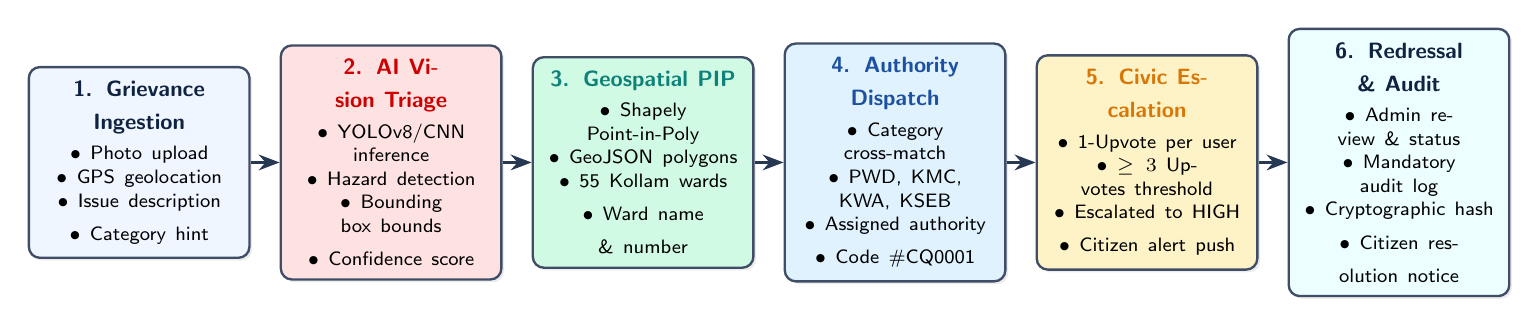
\begin{tikzpicture}[
    x=1cm, y=1cm,
    font=\sffamily,
    stepbox/.style={
        rectangle, draw=civNavy!80, line width=0.85pt, fill=white,
        rounded corners=4pt, inner sep=5pt, align=center,
        drop shadow={shadow xshift=1pt, shadow yshift=-1pt, opacity=0.15}
    },
    flowarr/.style={
        -{Stealth[scale=0.95]}, line width=1.1pt, draw=civNavy!90
    }
]

    % Step 1: Grievance Ingestion
    \node [stepbox, fill=cInput, text width=2.45cm] (p1) at (0, 0) {
        \textbf{\fontsize{8.5}{10.0}\selectfont\color{civNavy}1. Grievance Ingestion}\\[0.25em]
        \fontsize{7.2}{8.5}\selectfont
        $\bullet$ Photo upload\\
        $\bullet$ GPS geolocation\\
        $\bullet$ Issue description\\
        $\bullet$ Category hint
    };

    % Step 2: AI Vision Triage
    \node [stepbox, fill=cStage3, text width=2.45cm] (p2) at (3.20, 0) {
        \textbf{\fontsize{8.5}{10.0}\selectfont\color{red!80!black}2. AI Vision Triage}\\[0.25em]
        \fontsize{7.2}{8.5}\selectfont
        $\bullet$ YOLOv8/CNN inference\\
        $\bullet$ Hazard detection\\
        $\bullet$ Bounding box bounds\\
        $\bullet$ Confidence score
    };

    % Step 3: Geospatial PIP Mapping
    \node [stepbox, fill=cStage1, text width=2.45cm] (p3) at (6.40, 0) {
        \textbf{\fontsize{8.5}{10.0}\selectfont\color{civTeal}3. Geospatial PIP}\\[0.25em]
        \fontsize{7.2}{8.5}\selectfont
        $\bullet$ Shapely Point-in-Poly\\
        $\bullet$ GeoJSON polygons\\
        $\bullet$ 55 Kollam wards\\
        $\bullet$ Ward name \& number
    };

    % Step 4: Authority Dispatch
    \node [stepbox, fill=cStem, text width=2.45cm] (p4) at (9.60, 0) {
        \textbf{\fontsize{8.5}{10.0}\selectfont\color{civBlue}4. Authority Dispatch}\\[0.25em]
        \fontsize{7.2}{8.5}\selectfont
        $\bullet$ Category cross-match\\
        $\bullet$ PWD, KMC, KWA, KSEB\\
        $\bullet$ Assigned authority\\
        $\bullet$ Code \#CQ0001
    };

    % Step 5: Community Escalation
    \node [stepbox, fill=cStage2, text width=2.45cm] (p5) at (12.80, 0) {
        \textbf{\fontsize{8.5}{10.0}\selectfont\color{civGold}5. Civic Escalation}\\[0.25em]
        \fontsize{7.2}{8.5}\selectfont
        $\bullet$ 1-Upvote per user\\
        $\bullet$ $\ge 3$ Upvotes threshold\\
        $\bullet$ Escalated to HIGH\\
        $\bullet$ Citizen alert push
    };

    % Step 6: Resolution & Audit
    \node [stepbox, fill=cStage4, text width=2.45cm] (p6) at (16.00, 0) {
        \textbf{\fontsize{8.5}{10.0}\selectfont\color{civNavy}6. Redressal \& Audit}\\[0.25em]
        \fontsize{7.2}{8.5}\selectfont
        $\bullet$ Admin review \& status\\
        $\bullet$ Mandatory audit log\\
        $\bullet$ Cryptographic hash\\
        $\bullet$ Citizen resolution notice
    };

    % Connecting Flow Arrows
    \draw [flowarr] (p1) -- (p2);
    \draw [flowarr] (p2) -- (p3);
    \draw [flowarr] (p3) -- (p4);
    \draw [flowarr] (p4) -- (p5);
    \draw [flowarr] (p5) -- (p6);

\end{tikzpicture}
\end{document}
